% Draft manuscript. Target: Energy and Buildings / Applied Energy (Elsevier, elsarticle).
% Compile: pdflatex manuscript && bibtex manuscript && pdflatex manuscript && pdflatex manuscript
% (or upload the paper/ folder to Overleaf). Numbers marked \tbd{} are filled from results/ by the scripts.
\documentclass[preprint,12pt,authoryear]{elsarticle}
\usepackage{amsmath,amssymb,graphicx,booktabs,siunitx,hyperref,xcolor}
\newcommand{\tbd}[1]{\textcolor{red}{[#1]}}
\graphicspath{{../../results/figures/}}
\journal{Energy and Buildings}

\begin{document}
\begin{frontmatter}
\title{When does a hybrid adiabatic dry cooler save water? Coupled EnergyPlus simulation of wet/dry control
for data centers in 14 climates (DRAFT, companion paper)}
\author{Liang Zhang, Department of Civil and Architectural Engineering and Mechanics, University of Arizona, Tucson, AZ, USA \tbd{confirm affiliation}}
\begin{abstract}
\tbd{Draft. Split from the tower-evaporation manuscript after review round 1 (M1). Before submission, address the
open items listed in Section~\ref{sec:todo}.}
\end{abstract}
\end{frontmatter}

\section{Status of this draft}\label{sec:todo}
This section was split from the multi-method tower paper (review round 1, comment M1). The referee's hybrid-specific
concerns (M7) must be resolved before the results are used quantitatively:
\begin{enumerate}
\item The dry baseline cannot hold the condenser setpoint in hot climates, and chiller curves are clamped up to 12.8\,K
beyond their rated range (no EnergyPlus dataset chiller is valid above 41.1\,\textdegree C leaving condenser water). A high-lift
chiller characterisation (manufacturer data or a physics-based compressor model) is needed.
\item The tower and hybrid plants use different chillers; for energy comparisons both plants need the same chiller model.
\item Pad pressure drop is zero in the reported runs; pad effectiveness (0.85) and the design air rise (8\,K) are untested
assumptions. Add a sensitivity analysis and manufacturer pad data.
\item Equipment data now in hand (\texttt{docs/EQUIPMENT\_SPECS.md}, \texttt{data/equipment/evap\_pad\_performance.csv}) suggest:
pad effectiveness 0.75--0.80 for the base case (EVAPCO pad tests reach at most 78\,\% at 2\,m/s; a 150\,mm Munters pad is about
83\,\%); wet-pad pressure drop 20--85\,Pa; pad bleed of about 25\,\% of evaporation; manufacturer default switch-over to wet
only when fans are at 100\,\% and the setpoint is unmet, with a 21--26\,\textdegree C threshold, a lockout below
4\,\textdegree C and at most one wet start per day. The 0.02\,W/W fan power is reasonable (about Eurovent class C).
\item ``L/kWh saved'' ratios are unreliable where savings are small (0.03--0.08\,\%); report them only where savings exceed
a threshold, and express uncertainty.
\item Literature (verified, in references.bib): hybrid cooling towers \citep{asvapoositkul2014comparative}, pad
cooling efficiency and pressure drop \citep{he2014experimental}, spray pre-cooling \citep{alkhedhair2013numerical,yang2020experimental},
measured water use of pad pre-cooled condensers for data centres \citep{ndukaife2019optimization}; energy--water
trade-offs in hot--arid data centres \citep{karimi2022water,karimi2025energy}.
\item Control uses perfect knowledge of the current dry-bulb; add dwell time, demand-based control, pad flushing/start-up
water and freeze protection.
\end{enumerate}

%======================================================================
\section{Hybrid adiabatic dry coolers}\label{sec:hybrid}
%======================================================================
\subsection{Model}
Hybrid (adiabatic) dry coolers are the main water-saving alternative to towers in new data centers. EnergyPlus has
dry fluid coolers but no water-side hybrid cooler, so the plugin builds one: a bank of \texttt{FluidCooler:TwoSpeed}
objects shares one outdoor-air node, and in wet mode the plugin overrides that node's dry-bulb with the pad-leaving
temperature, keeping the wet-bulb, through EMS actuators at the start of each timestep. EnergyPlus then simulates the
coils with pre-cooled air, and a condenser setpoint manager that follows the node lowers the condenser water
temperature, so the chillers see the benefit. Pad cooling follows adiabatic saturation,
\begin{equation}
T_{pre} = T_{db} - \varepsilon\,(T_{db}-T_{wb}),\qquad i(T_{db},\omega_i) + (\omega_{pre}-\omega_i)c_{pw}T_{wb} = i(T_{pre},\omega_{pre}),
\end{equation}
with pad effectiveness $\varepsilon=0.85$ (assumption, typical of rigid media). Evaporation is
$E=\sum_k f_k\dot m_{a,k}(\omega_{pre}-\omega_i)$ over the fan states of the timestep, recovered exactly from the
coolers' reported fan power, and bleed follows the chemistry model of the companion paper. Unlike the tower
analysis, this plugin changes the EnergyPlus solution.

\subsection{Case study and control strategies}
The data-center model of the companion paper was given a hybrid heat-rejection plant: three 50\,\% fluid coolers
(N+1) sized for wet operation at the 0.4\,\% dry-bulb design condition (5.6\,K approach and range, 8\,K design air
temperature rise, hard-sized air flows), a condenser setpoint of pad-leaving air plus 5.6\,K (23--40\,\textdegree C), and
three 50\,\% inlet-vane centrifugal chillers (Trane CVHE curve set, rated COP 5.38). No chiller curve set in the
EnergyPlus dataset is valid above 41.1\,\textdegree C leaving condenser water; hours beyond that limit, where EnergyPlus
clamps the curves and underestimates chiller energy, are reported for every case. Seven control strategies were run
at all 14 sites on identical hardware: dry only, always wet (above 5\,\textdegree C), and wet when the outdoor
dry-bulb exceeds $T_{on}=$ 16, 20, 24, 28 or 32\,\textdegree C (2\,K hysteresis). Because the tower and hybrid plants use
different chiller curve sets, energy is compared only among hybrid strategies, and the tower enters as a water
reference.

\subsection{Results}
Table~\ref{tab:hybrid} and Figs.~\ref{fig:hybtrade}--\ref{fig:hybwue} summarise the results. Three findings stand out.

\emph{Wet operation is primarily a capacity measure.} Dry-only, the chillers run beyond their rated condenser range
for up to 3,285\,h/yr (Riyadh), 2,800\,h (Phoenix) and 1,170--1,880\,h in Dallas, Houston, Mumbai and Singapore. Wetting above
28\,\textdegree C reduces this to at most 5\,h/yr at every site.

\emph{Saving electricity with pad water is expensive.} Relative to dry operation, wetting above 28\,\textdegree C saves 0--1.7\,\%
of facility electricity at a marginal cost of 100--122\,L of water per kWh saved, and always-wet operation 107--241\,L/kWh.
These figures overstate the cost somewhat, because the dry baseline's chiller energy is underestimated where curves clamp.

\emph{Control decides whether a hybrid saves water.} With wetting above 28\,\textdegree C, site water is 14\,\% (Riyadh),
31\,\% (Phoenix) and 41\,\% (Las Vegas) lower than the evaporative tower, 60--85\,\% lower in hot--humid climates, and
93--100\,\% lower in cool climates. Always-wet operation in Riyadh uses 9\,\% \emph{more} water than the tower, because the
pads cool all the air the dry coil moves, which is more air than a wet tower needs for the same heat.

\begin{figure}[t]\centering
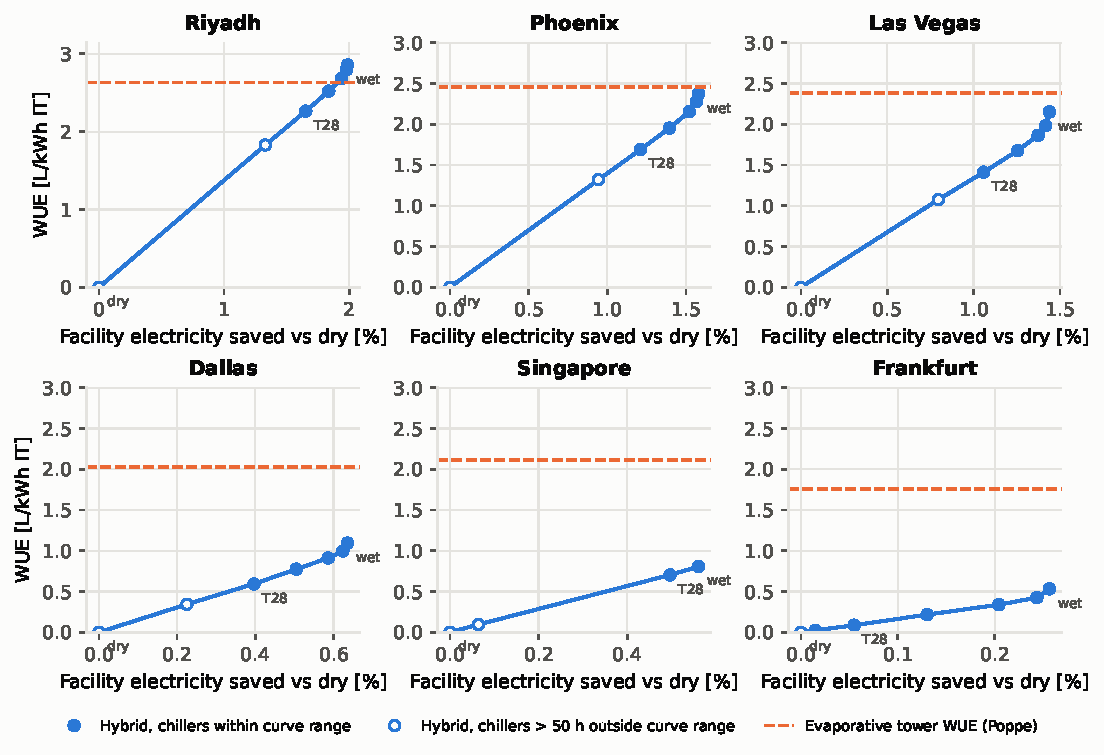
\includegraphics[width=\linewidth]{fig_hybrid_tradeoff}
\caption{Water--energy trade-off of hybrid dry-cooler control (dry, wet above 32 to 16\,\textdegree C, always wet) at six
sites; dashed: evaporative tower WUE at the same site. Open markers: chillers more than 50\,h/yr outside their rated curve range.}\label{fig:hybtrade}
\end{figure}

\begin{figure}[t]\centering
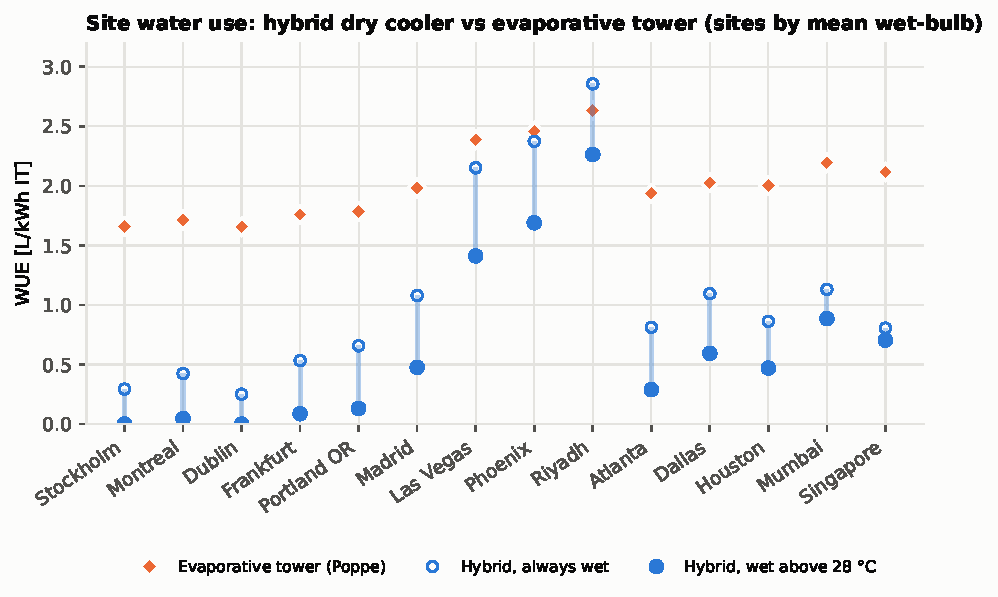
\includegraphics[width=\linewidth]{fig_hybrid_wue}
\caption{Site water use of the hybrid dry cooler (wet above 28\,\textdegree C and always wet) and the evaporative tower.}\label{fig:hybwue}
\end{figure}

\begin{table}[t]\centering\scriptsize
\caption{Hybrid dry cooler results by site (sorted by mean wet-bulb). WUE in L/kWh IT; $\Delta$WUE$_{T28}$ relative to the tower;
h$_{out}$: chiller hours outside rated curve range; $\Delta E_{T28}$: facility electricity saved vs dry; L/kWh$_{saved}$: water
per kWh saved (T28).}\label{tab:hybrid}
\resizebox{\linewidth}{!}{\begin{tabular}{llrrrrrrrr}
\toprule
Site & CZ & WUE$_{tower}$ & WUE$_{T28}$ & WUE$_{wet}$ & $\Delta$WUE$_{T28}$ [\%] & h$_{out}$ dry & h$_{out}$ T28 & $\Delta E_{T28}$ [\%] & L/kWh$_{saved}$ \\
\midrule
Stockholm & 6A & 1.66 & 0.00 & 0.29 & -100 & 0 & 0 & 0.00 & -- \\
Montreal & 6A & 1.72 & 0.05 & 0.42 & -97 & 35 & 0 & 0.03 & 114 \\
Dublin & 5A & 1.66 & 0.00 & 0.25 & -100 & 0 & 0 & 0.00 & -- \\
Frankfurt & 4A & 1.76 & 0.09 & 0.53 & -95 & 78 & 0 & 0.05 & 120 \\
Portland OR & 4C & 1.79 & 0.13 & 0.66 & -93 & 115 & 0 & 0.08 & 122 \\
Madrid & 3B & 1.98 & 0.48 & 1.08 & -76 & 648 & 0 & 0.33 & 109 \\
Las Vegas & 2B & 2.39 & 1.41 & 2.15 & -41 & 2185 & 0 & 1.06 & 100 \\
Phoenix & 1B & 2.46 & 1.69 & 2.37 & -31 & 2803 & 3 & 1.21 & 104 \\
Riyadh & 1B & 2.63 & 2.26 & 2.86 & -14 & 3284 & 0 & 1.65 & 102 \\
Atlanta & 3A & 1.94 & 0.29 & 0.81 & -85 & 457 & 0 & 0.20 & 109 \\
Dallas & 2A & 2.03 & 0.59 & 1.09 & -71 & 1226 & 1 & 0.40 & 113 \\
Houston & 2A & 2.00 & 0.47 & 0.86 & -77 & 1172 & 5 & 0.30 & 116 \\
Mumbai & 0A & 2.19 & 0.89 & 1.13 & -60 & 1875 & 4 & 0.59 & 112 \\
Singapore & 0A & 2.12 & 0.70 & 0.81 & -67 & 1208 & 4 & 0.50 & 105 \\
\bottomrule
\end{tabular}
}
\end{table}


\section*{Data and code availability}
The hybrid-cooler plugin, models and scripts are available at
\url{https://github.com/TensorBuildLab/EnergyPlus-HeatRejection-Water} under the MIT licence.

\bibliographystyle{elsarticle-harv}
\bibliography{../references}
\end{document}
